% THIS IS SIGPROC-SP.TEX - VERSION 3.1
% WORKS WITH V3.2SP OF ACM_PROC_ARTICLE-SP.CLS
% APRIL 2009
%
% It is an example file showing how to use the 'acm_proc_article-sp.cls' V3.2SP
% LaTeX2e document class file for Conference Proceedings submissions.
% ----------------------------------------------------------------------------------------------------------------
% This .tex file (and associated .cls V3.2SP) *DOES NOT* produce:
%       1) The Permission Statement
%       2) The Conference (location) Info information
%       3) The Copyright Line with ACM data
%       4) Page numbering
% ---------------------------------------------------------------------------------------------------------------
% It is an example which *does* use the .bib file (from which the .bbl file
% is produced).
% REMEMBER HOWEVER: After having produced the .bbl file,
% and prior to final submission,
% you need to 'insert'  your .bbl file into your source .tex file so as to provide
% ONE 'self-contained' source file.
%
% Questions regarding SIGS should be sent to
% Adrienne Griscti ---> griscti@acm.org
%
% Questions/suggestions regarding the guidelines, .tex and .cls files, etc. to
% Gerald Murray ---> murray@hq.acm.org
%
% For tracking purposes - this is V3.1SP - APRIL 2009

\documentclass{acm_proc_article-sp}

\usepackage[utf8]{inputenc}

\newcommand{\carbondioxide}{\ensuremath{\mathrm{CO}_2}}
\newcommand{\eqdef}{\ensuremath{\overset{\mathrm{def}}{=}}}

\begin{document}

\title{Cooling-aware Geographical Load Balancing Visualized\titlenote{This research is supported by the NSF, Mr. David C. Elliot's family, and the Rose Hills Foundation.}}
\numberofauthors{4}
\author{
% You can go ahead and credit any number of authors here,
% e.g. one 'row of three' or two rows (consisting of one row of three
% and a second row of one, two or three).
%
% The command \alignauthor (no curly braces needed) should
% precede each author name, affiliation/snail-mail address and
% e-mail address. Additionally, tag each line of
% affiliation/address with \affaddr, and tag the
% e-mail address with \email.
%
% 1st. author
\alignauthor
Michael Hirshleifer\\
	\affaddr{California Institute of Technology}\\
	\affaddr{1200 E California Blvd}\\
	\affaddr{Pasadena, California}\\
	\email{111mth@caltech.edu}
% 2nd. author
\alignauthor
Yizhen Wang\\
	\affaddr{California Institute of Technology}\\
	\affaddr{1200 E California Blvd}\\
	\affaddr{Pasadena, California}\\
	\email{ywang3@caltech.edu}
\and
% 3rd. author
\alignauthor
Zhenhua Liu\\
	\affaddr{California Institute of Technology}\\
	\affaddr{1200 E California Blvd}\\
	\affaddr{Pasadena, California}\\
	\email{zliu2@caltech.edu}
% the prof
\alignauthor
Adam Wierman\\
	\affaddr{California Institute of Technology}\\
	\affaddr{1200 E California Blvd}\\
	\affaddr{Pasadena, California}\\
	\email{adamw@caltech.edu}
}

\date{2012-10-02}

\maketitle
\begin{abstract}
We explore how geographical load balancing can improve the efficiency of renewable energy use in data centers.
The model incorporates varying cooling efficiency (considering weather conditions) and electricity prices over time at each data center.
We run a convex optimization over routing, using as input real workload, temperature, solar, and wind traces.
We find that using geographical load balancing lets data centers more effectively use locally available renewable energy, thereby substantially reducing their usage of grid electricity. This conclusion holds across seasons.
We develop a visualization that displays the demand from each of the 48 contiguous U.S. states and the energy usage, grid energy usage, and renewable energy generation at each of 10 data centers, animated over time according to the input data and the optimization output. The resulting software can be used to test effectiveness of and refine routing algorithms.
\end{abstract}

\section{Introduction}


\subsection{The problem}
	\subsubsection{Energy cost is important for DCs.}
		Building cost-saving and environmentally-friendly data centers has become a pressing challenge for the ICT industry.
		Energy consumption accounts for much of a data center’s running cost \cite{datacenter}, and the carbon dioxide emissions consequent to data centers’ grid energy usage concerns society at large.
		As the need for data centers grows rapidly,
		“green” routing algorithms would benefit internet companies by reducing their electricity costs, and everyone else by reducing pollution from non-renewable energy. The social benefit could be substantial, as data centers are expected to use several percent of U.S. and world electricity output, and they currently use mostly non-renewable energy.
		
		\paragraph{Servers use energy to process requests}
			Data centers require a substantial amount of energy, both for processing requests and for cooling. The energy the servers themselves use to process requests varies with load (requests processed per second).
		\paragraph{Cooling also uses energy}
			Data centers also spend a considerable amount of energy on cooling \cite{datacenter}, especially in summer. The energy needed for cooling largely depends on the weather at data center locations. Thus we can also exploit the geographical heterogeneity of the data centers to reduce cooling cost.
	\subsubsection{Load balancing between DCs}
		There are often several redundant data centers, each of which can process a user request, such as a Google search. Traditionally, a request would be routed to the geographically-nearest data center, thereby minimizing latency—without considering energy efficiency.
	\subsubsection{Load, energy availability, grid electricity prices, etc. are time-varying and stochastic.}
		\paragraph{Renewable vs. grid energy}
			Currently, data centers are powered mainly by buying electricity off the grid. Grid electricity necessarily comes substantially from burning fossil fuels, because with current technology, storing renewable energy over time to match demand is prohibitively expensive.
			
			However, some data centers are already partly operated on green energy. Data centers may have dedicated renewable energy generation (solar or wind farms). But the renewable power output at each location varies over time (time of day, cloud cover, wind speed), and generally does not match user demand, so excess demand must be satisfied by buying electricity off the grid.


\subsection{Previous work}
	\subsubsection{Geographical load balancing}
		Flexibility in routing could allow a network of data centers to run almost entirely off renewable energy. When routing a request, there is a trade-off: instead of always choosing the nearest data center, a request can be routed to a data center where renewable energy is currently being produced (reducing electricity costs), at the expense of somewhat higher latency. Professor Wierman’s group have devised optimal or near-optimal (given a functional form for the business cost of increased latency) routing algorithms for efficient geographical load balancing.
		\paragraph{Can use almost entirely renewables}
			Previous research suggests that under the geographical load balancing (GLB) model, the system of data centers can even operate almost entirely on renewable energy, without undue increase in latency \cite{adam:GLB}.
		\paragraph{Convex optimization framework; solve numerically}
			Our simulation models the whole data center routing system, using real-world data on wind and solar power output, grid electricity prices, and internet request volume over time at various locations (the 48 contiguous U.S. states and 10 data center locations). The simulation is implemented as a convex optimization problem, solved numerically, whose solution is an allocation of requests to data centers.
		
		@@@@@The previous GLB model [@@@citation] only considers the energy cost of running the servers. But in reality, a data center spends a considerable amount of energy on cooling


\subsection{Visualization}
We implement a comprehensible visualization of the multi-dimensional simulation input and output data. The visualization makes it easier to see what each optimization algorithm is doing, so it can be used to test effectiveness of and refine routing algorithms. This will help develop the end goal of an implementable algorithm / system for routing internet requests that allows data centers to operate using almost exclusively renewable energy.

\subsection{Cooling-aware GLB}

This paper shows that a new geographical load balancing model which considers energy cost in cooling is able to reduce the total cost significantly compared to previous models. This improvement in green energy usage leads to much lower carbon emissions.

We set up an experiment to investigate the economic and environmental impact of our new model. We use real traces of data center workload, renewable energy availability, and weather to numerically compute the optimal solution.% The cost model of the geographical load balancing system is analytically determined@@@@[what that mean lah].

Our study leads to three major findings.

First, the new GLB model, the Cooling-aware GLB model, reduces the total cost of the system. This is because it is able to distribute the request to locations with not only cheap energy, but also favorable weather for cooling. More excitingly, the optimal cost does not vary much with seasonality. This can potentially solve the problem of data center cooling in places with climate and weather extremes (like strong diurnal temperature variation).

Second, the Cooling-aware GLB model can allow significantly reduced carbon emissions, halved compared to the previous models. The new GLB model makes better-informed decisions than the previous GLB model by considering the energy for cooling.

Third, considering cooling yields a larger benefit than adding energy storage, both in total cost and in carbon emissions, provided that the aggregate renewable supply is enough to power the data centers yet not in vast surplus. We obtain this result by systematically comparing the Cooling-aware GLB system with storage systems of various storage capacities. We conclude that Cooling-aware GLB has a clear advantage over the storage model when the renewable energy generation and storage facilities are not widely established; it requires much less investment in infrastructure and hence can be implemented more easily.

\section{Setup}
We assume that each data center has a cooling system described in \cite{adam:cooling}, and then modify the model in \cite{adam:GLB} to include energy cost of cooling. The model can be solved using convex optimization technique as proved in \cite{adam:GLBfull}.
\subsection{The workload}
Let $J$ be the set of sources of requests. Each of 48 U.S. states is modeled as having a source of web requests located at its geographical center. The request volume is $L_j(t)$, the mean arrival rate from source $j \in J$ at time interval $t$. $L_j(t)$ is estimated using real-world traces. The base trend of the workload is taken from a trace at Hewlett-Packard Labs, then the workload of each request source is scaled proportionately to the population of the state, following by a shift along the time dimension according to the timezone.

\subsection{The availability of renewable energy}
We have three major considerations when modeling the availability of renewable energy:

First, the weather at the data centers is crucial, as it determines the renewable energy output. We use real traces of wind speed and insolation obtained from \cite{renew1} \cite{renew2}.
%@@@@@@[Is this true? I thought the traces were (calculated) power output.]
The measurements have a granularity of 10 minutes. The rate of renewable energy generation per plant unit at each data center is then set to be proportional to the weather data respectively.

Second, the size of the renewable energy plant matters. We scale the renewable generation capacity such that the total renewable energy is $c$ times as much as the total energy demand to process all requests. In our simulation, $c$ varies in $[0.5, 4]$ with a step length of $0.5$.

Third, we must choose an optimal mix of solar and wind energy to power the data centers. Previous research \cite{adam:GLB} suggests that a mix of 80\% of wind and 20\% of solar fits the data center energy consumption characteristics nicely. We adopt this ratio in our simulation throughout.
%%%%%%%%%%%%%%%%%%%%
\subsection{The internet-scale system}
The internet-scale system consists of a set $\mathcal{N}$ of 10 data centers at Google data center locations in California, Washington, Oregon, Illinois, Georgia, Virginia, Texas, Florida, North Carolina, and South Carolina. The number of servers (or equivalently, processing capacity) $X_i$ at data center $i$ is set to be twice the peak load at $i$ when all requests are routed to the nearest data centers.

The optimization will determine the routing plan $\lambda_{ij}(t)$ and the number of active servers $x_i(t)$ that minimizes the total cost (the sum of delay cost, energy cost, and switching cost).

\subsubsection{Delay cost}
The delay cost represents the revenue loss incurred due to delay in processing requests. It comprises the propagation delay $d_{ij}$ from source $j$ to date center $i$ and the queuing delay at $i$.
The propagation delay $d_{ij}$ is calculated to be the time needed to travel between $i$ and $j$ at a transmission speed of $200 \frac{\mathrm{km}}{\mathrm{ms}}$ plus a constant term $5 \mathrm{ms}$. The queuing delay is calculated from the parallel M/G/1/Processor Sharing queue model in which the total load $\lambda_i(t)=\sum_j \lambda_{ij}(t)$ is distributed evenly across $x_i(t)$ homogeneous servers of service rate \mbox{$\mu_i$ = $0.1 / \mathrm{ms}$}.

\subsubsection{Cooling optimization}
The cooling optimization model finds the minimum energy consumption required to maintain the data center at constant temperature $T = 25^{\circ}\textrm{C}$. A typical data center uses both air cooling and chilled-water cooling. Let $x = x_a + x_c$ be the total number of active servers, $x_a$ the number of those that are air-cooled, and $x_c$ the number cooled with chilled water. This model finds the best division between $x_a$ and $x_c$.

The energy consumption of air cooling is
\begin{equation}
c_a(x_a) = k \cdot {x_a}^3, 0 \leq x_a \leq \bar{x}, k > 0
\end{equation}
The parameter $k$ is proportional to the temperature gradient between the inside and outside air. The parameter $\bar{x}$ corresponds to the maximum number of the servers that can be cooled by air cooling alone. The cap $\bar{x}$ is proportional to both the temperature gradient and the maximum air flow rate. In our simulation, the air flow rate is set such that when the outside temperature is $20^{\circ}\mathrm{C}$ lower than $T$, the data center can rely on air cooling entirely at full workload.

On the other hand, the energy consumption of chilled-water cooling is empirically roughly linear in the IT demand, so we model it as
\begin{equation}
c_c(x_c) = \gamma \cdot x_c
\end{equation}
%Here $\gamma = 0.17$, meaning that the chiller takes 0.17kW/h electricity to cool the heat caused by 1kw/h of IT demand.

For notational convenience, define
\begin{equation}
	u^+ \eqdef \max(0, u)
\end{equation}
to be $u$ clamped to be nonnegative.

The optimal cooling portfolio is
\begin{equation}
c(x) = \min_{x_a \in [0,x]}\left( \gamma \cdot (x-x_a)^+ + k \cdot {x_a}^3 \right)
\end{equation}
which yields
$$
c(x) = \left\{ \begin{array}{ll}
	k \cdot x^3 & \mbox{if $x \geq x_s$}\\
	k \cdot x_s^3 + \gamma \cdot (x-x_s) & \mbox{otherwise}\end{array} \right.
$$
where $x_s = \min \left(\sqrt{\gamma/3k}, \bar{x}\right)$ is the threshold for when chiller cooling is necessary.

To explore the effect of seasonality on the performance of the cooling model, we use two sets of temperature data. One is taken from the first week of January 2012 from \cite{temp}; the other is take from the first week of July 2012. The measurements are taken hourly.

\begin{figure*}
\centering
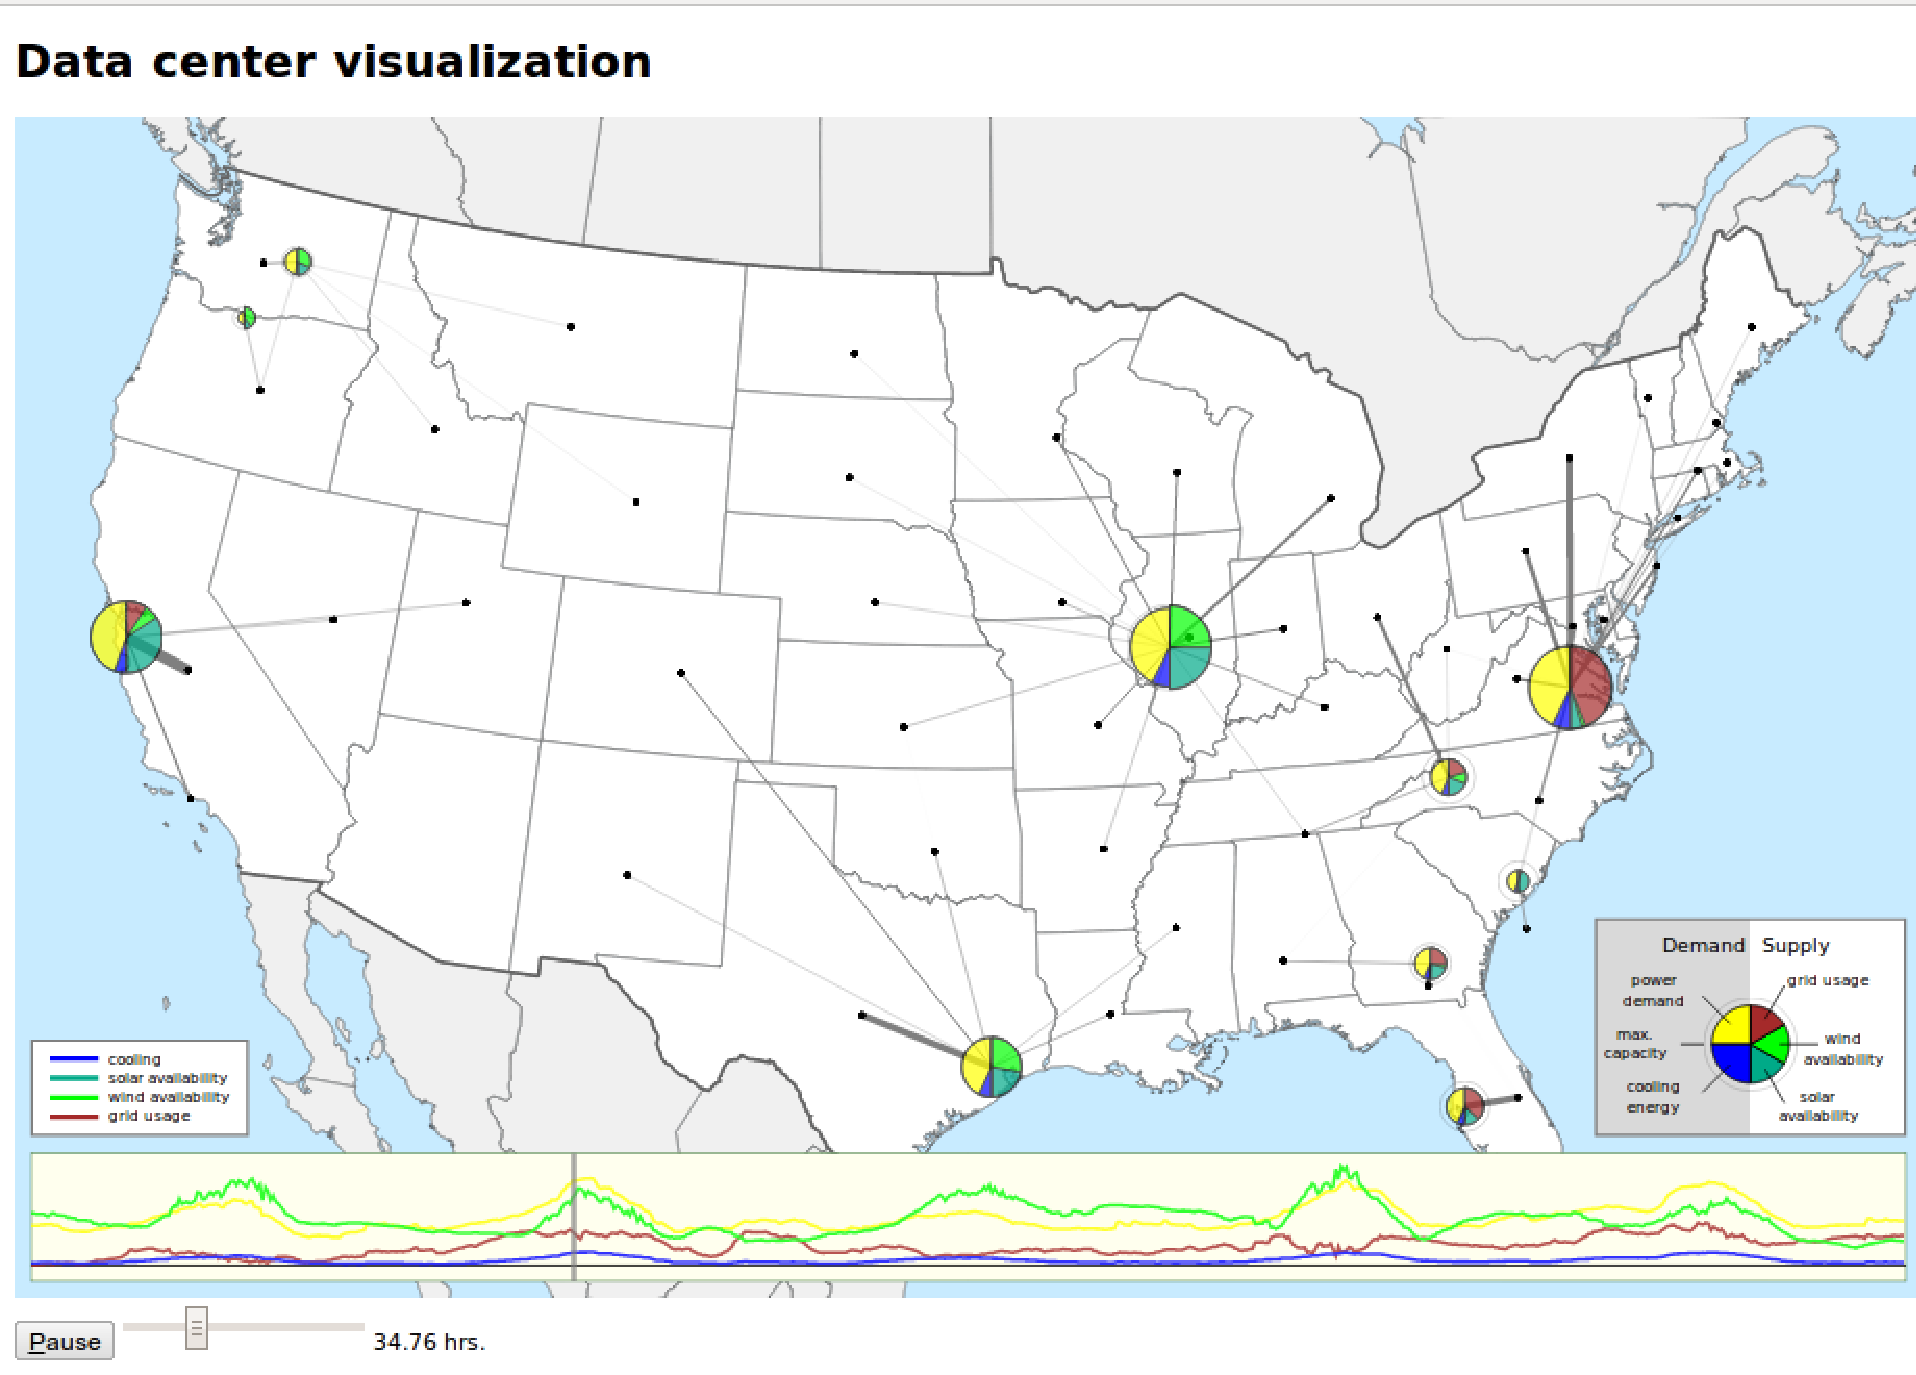
\epsfig{file=visualization-bmp.pdf, height=3in, width=4.5in}
\caption{Screenshot of the visualization, running in the Chromium web browser.}
\end{figure*}
\subsubsection{Energy cost}
The energy cost is the cost of both running active servers and keeping them at constant working temperature. The data centers pay no cost for renewable energy; we assume that each data center has dedicated renewable energy generation facilities that incurs zero maintenance cost. Thus the energy cost is for using energy from the grid and can be represented as
\begin{equation}
p_i \cdot (l(x_i(t)) + c(x_i(t)) - r_i(t))^+
\end{equation}
where $p_i$ is the price of electricity; $x_i(t)$ is the number of active servers at that time interval $t$; $l(x_i(t))$ is energy consumption of active servers themselves in the time interval, or IT demand; $c(x_i(t))$ is the energy usage for cooling; and $r_i(t)$ is the renewable energy availability. In our model, $p_i$ is set to be constant according to the real statistics of each state; $l$ is a linear function of $x(t)$.

\subsubsection{Switching cost}
The switching cost models the delay and wear-and-tear cost when switching on/off servers. In our model, the workload at each data center is updated every 10 minutes. To avoid excessively-frequent switching of server status, we define the switching cost to be
$$\beta \cdot (x_i(t+1) - x_i(t))^+$$
where $\beta$ is the weight of switching cost. In our simulation, $\beta = 6$.

\subsubsection{Storage}
In addition to renewable-energy generators, data centers may also install energy storage (in the form of batteries, supercapacitors, flywheels, etc.). Renewable-energy availability varies greatly over time; introducing storage smooths out the supply.

We model the amount of electricity storage at time $t$ to be $0 \leq es_i(t) \leq ES_i$, where $ES_i$ is the maximum storage capacity. Let the storage rate be
$$e_i(t) = \rho \cdot (es_i(t) - es_i(t+1))$$
Positive $e_i(t)$ means discharging, negative charging. The parameter $\rho$ represents the charging and discharging efficiency. In our simulation we assume perfect efficiency, i.e. $\rho = 1$.

In the presence of storage, the energy cost is
\begin{equation}
p_i \cdot (l(x_i(t)) + c(x_i(t)) - r_i(t) - e_i(t))^+
\end{equation}

\subsubsection{Total cost}
Now we can formally write our optimization problem as:
\begin{align*}
\min_{\bf{x}(t), \bf{\lambda}(t)} & \sum_{i \in \mathcal{N}} p_i \cdot (l(x_i(t)) + c(x_i(t)) - r_i(t) - e_i(t))^+ \\
& + \sum_{j \in \mathcal{J}}\sum_{i \in \mathcal{N}}
\lambda_{ij}(t)\left(\frac{1}{\mu_i - \lambda_i(t)/x_i(t)} + d_{ij}\right) \\
& + \beta \cdot (x_i(t+1) - x_i(t))^+
\end{align*}
subject to
\begin{align*}
& \sum_{i\in \mathcal{N}}\lambda_{ij}(t) = L_j(t), &\forall j\in J \\
& \lambda_{ij} \geq 0, & \forall i\in N, j\in J \\
& 0 \leq x_i(t) \leq X_i, & \forall i \in N \\
& \lambda_i(t) \leq x_i(t) \cdot \mu_i & \forall i \in N \\
& 0 \leq es_i(t) \leq ES_i & \forall i \in N \\
& e_i(t) = es_i(t) - es_i(t+1) & \forall i \in N
\end{align*}

The boundary conditions model the following real-world constraints:
\begin{enumerate}
\item
The requests from a population center all have to be processed by the geographical load balancing system. Each data center should receive a non-negative amount of work.
\item
Each data center has a limited number of servers; it cannot process requests in excess of its computational capacity.
\item
Each data center's energy storage capacity is bounded between $0$ and a fixed cap.
\end{enumerate}
\subsubsection{\carbondioxide{} emission}
The optimization thus far has the sole objective of minimizing the cost to the firm. But we also want to monitor the amount of \carbondioxide{} emitted as an externality. The emission of \carbondioxide{} arises from grid electricity use; the emissions rate per kW$\cdot{}$h varies across states, as each state has a different energy-source composition. An estimation of these rates can be found at \cite{carbon}.

Let $\eta_i$ be the rate of carbon emission per kW/h at data center $i$, the total \carbondioxide{} emission is then
$$\sum_{i \in \mathcal{N}} \eta_i \cdot (x_i(t) + c(x_i(t)) - r_i(t) - e_i(t))^+$$
\subsubsection{Benchmarks for comparison}
Our model is the first to integrate practical cooling concerns into geographical load balancing. To show their impact, we will compare the result of our model (Cooling-aware GLB) to the previous Cooling-Oblivious GLB model and the model which simply routes all requests to the nearest data centers (LOCAL). For the two benchmark models, the cooling optimization is done after the routing scheme is determined.

Separately, we compare the performance of our model to the storage model. Storage capacity is quantified as the duration that a data center could operate at maximum load entirely off stored energy (excluding energy usage for cooling). We assume that storage incurs no running cost. We choose data-center systems with 3-hour and 6-hour storage respectively as the benchmark.

We will evaluate the outcomes based on 1) the total cost; 2) the grid (brown) energy usage; and 3) the \carbondioxide{} emissions.

\begin{figure*}
\centering
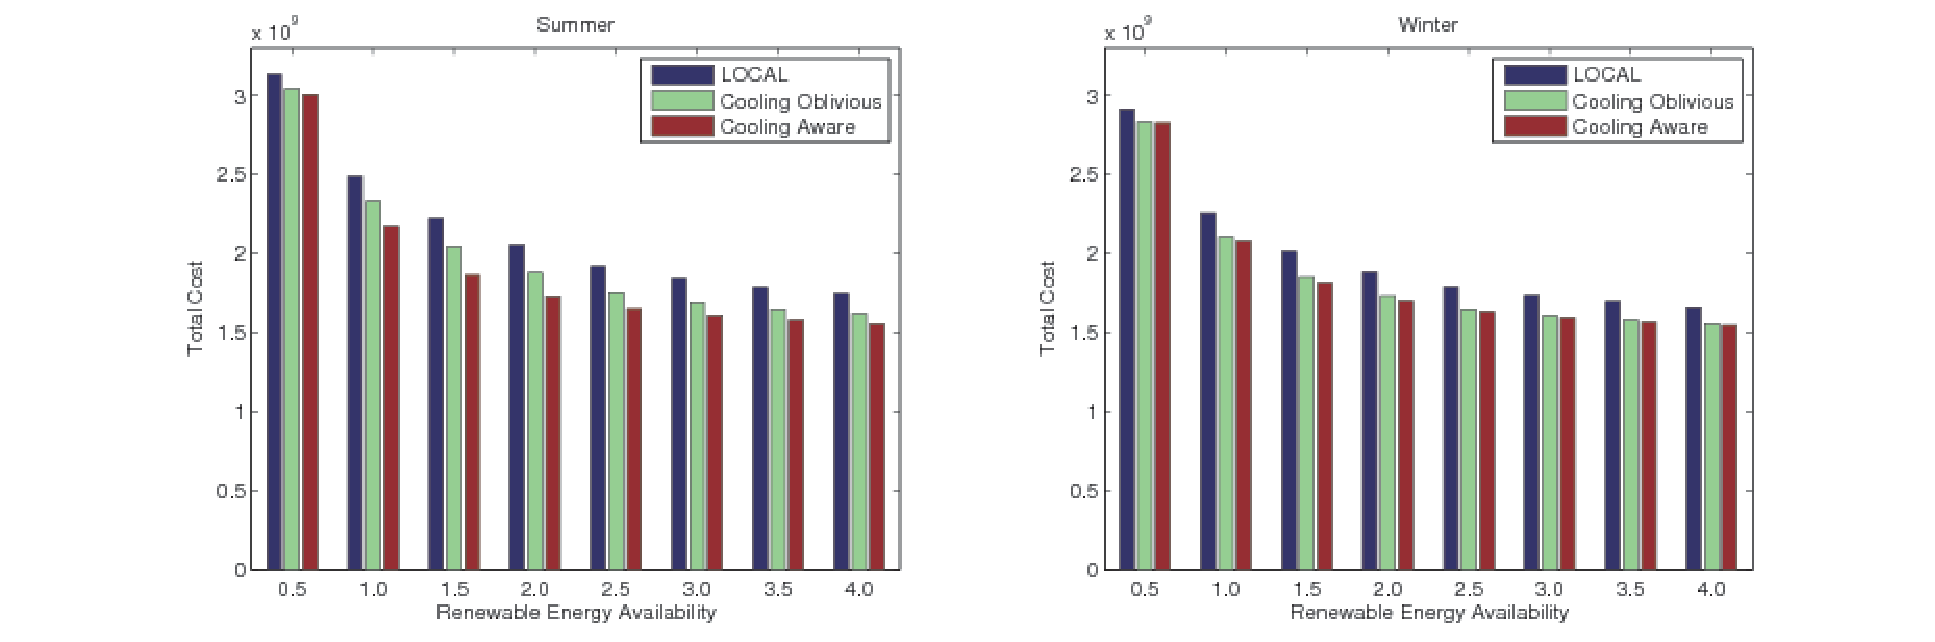
\epsfig{file=cost_comparison.pdf, height=1.8in, width=7in}
\caption{Comparison of optimal costs of Cooling-aware GLB, Cooling-oblivious GLB and LOCAL, with varying renewable energy availability.}
\end{figure*}
\section{Visualization}
Our numerical experiment generates time series describing routing plans and data center activity. Due to the large quantity of data, the output is hard to interpret when in matrix form. Therefore we developed a visualization tool to help us recognize the key characteristics of the optimal solution quickly. It also works as a simple check for the validity of the solution: we can spot obviously abnormal behaviors in the output.

\subsection{Technical description}
The output visualization is in Scalable Vector Graphics (SVG) format, a high-quality XML-based vector graphics format supporting fluid animations that display time-series data. This animation can be embedded into a web page.

We also wrote a wrapper XHTML web page to make the simulation easier to use. The user can control the animation (play, pause, or seek into the animation) using the interface on the web page (implemented using Javascript). Possible enhancements could include zooming, panning, and showing/hiding types of map elements.

Both components work in the Chromium web browser and pass the W3C validators.

The back-end script that generates the SVG map from input data is written in the Scala programming language. The script reads in and displays data center locations, client (request source) locations, real solar- and wind-generation traces, and the routings optimized according to the various algorithms (from the output of the Matlab optimizations). We are provided the raw input data in CSV format; Matlab outputs are exported to the NetCDF format for reading into Scala.

We use as a background a map \cite{wikimap} of the 48 contiguous United States obtained from Wikimedia Commons. Points on the map correspond to real-world $(latitude, longitude)$ coordinates according to a mathematical transformation specified with the map; this allows us to draw physical locations at the correct positions on the map.

\subsection{Graphical representation details}
The visualization page consists of three components: an animation showing the dynamic status of the geographical load balancing system, a line plot showing the aggregate statistics of energy supply and demand, and a progress bar allowing progress scroll and control.

The animation displays 10 data centers on a base map of the United States. Each data center's status is represented by a sector diagram, which is animated over time. The left half of the circle represents the energy demand of the data center: the yellow sector is the energy demand for processing the request, the blue one the energy demand for cooling. The right half of the circle represents the energy supply: the light green sector represents available wind energy, the dark green one represents available solar energy, and the brown one represents the energy usage from the grid. The area of each sector is proportional to the amount of energy (so its radius is proportional to the square root). In addition, each sector diagram is surrounded by a faint circle, which represents the maximum energy usage when the data center operates at full load.

The request traffic $\lambda_{d,s}(t)$ is represented by lines connecting each source $s$ and destination data center $d$. The width of the line is linearly proportional to $L_s(t)$, the total volume of requests from $s$. The transparency of the line is linearly proportional to ${\lambda_{d,s}(t)} / {L_s(t)}$, the percentage of the traffic from the source $s$ routed to each data center. A solid black line means all the requests from $s$ are sent to $d$, while a fully transparent line means that no traffic is routed from $s$ to $d$.

The line plot displays four aggregate statistics of interest over time: the yellow line shows the aggregate IT power, the blue one the aggregate energy usage on cooling, the light green one the aggregate wind energy available, and the dark green one the aggregate solar energy available.

The progress bar at the bottom indicates the time elapsed in the animation. The user can pause/resume the animation and seek to the desired time.


\section{Results}
\subsection{Cost savings from Cooling-aware GLB}

\begin{figure}
\centering
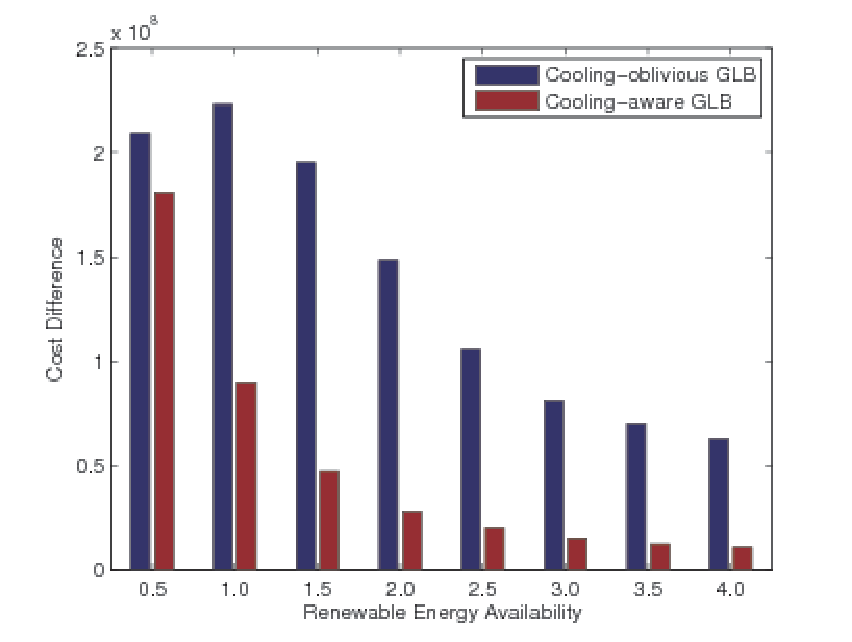
\epsfig{file=cost_diff.pdf, height=2.2in, width=3.2in}
\caption{The difference between optimal costs in summer/winter for both Cooling-aware and Cooling-oblivious GLB}
\end{figure}

The cooling-aware geographical load balancing model reduces firm's energy cost by routing the requests to locations where energy is cheap and cooling is easy. Such a savings outweighs the increase in delay cost. Hence our model is consistent profit maximization by a firm.

%In this experiment, the aggregate amount of renewable energy is set to be the total IT demand multiplied by a coefficient, where the coefficient series is the integer multiples of 0.5 within [0.5, 4]. We run the experiment under both summer and winter weather.

Our first experiment explores the cost efficiency of the this model. Figure 2 illustrates the extent of total cost savings of our model. We choose the total cost under Cooling-oblivious GLB and LOCAL as the benchmark. The Cooling-aware model gives lower cost than both benchmarks. This edge is rather clear under two situations. First, in summer when cooling is expensive, the Cooling-aware model significantly outperforms Cooling-oblivious model; by considering the energy cost of cooling, it makes routing decisions to use renewable energy optimally. Second, when the aggregate renewable energy available lies between once and twice the aggregate demand, and some but not all data center locations have a surplus in renewables, the Cooling-aware GLB exploits this surplus better than the benchmarks.

We are interested in how well the Cooling-aware GLB model works in different seasons and weather conditions. Figure 3 shows the difference between the optimized costs in summer and in winter using each model. The previous Cooling-oblivious model's performance varies significantly with seasonality; our Cooling-aware GLB model's performance is more robust. This finding suggests that our Cooling-aware model exploits the heterogeneity in weather to reduce the energy required for cooling.
%\begin{figure}
%\centering
%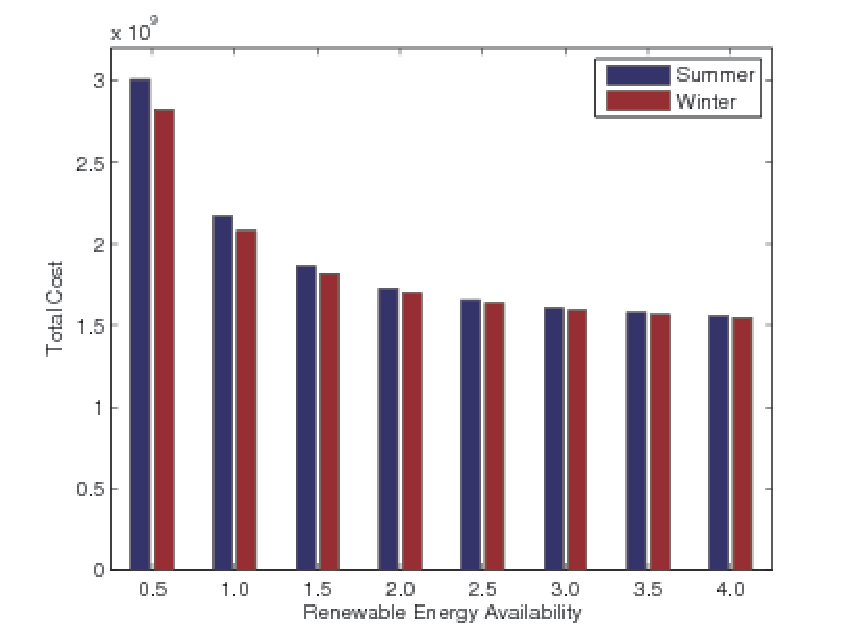
\epsfig{file=opt_cost_comparison.pdf, height=2.2in, width=3.2in}
%\caption{A sample black and white graphic (.eps format).}
%\end{figure}



\subsection{Environmental impact - \carbondioxide{} savings}


\begin{figure}
\centering
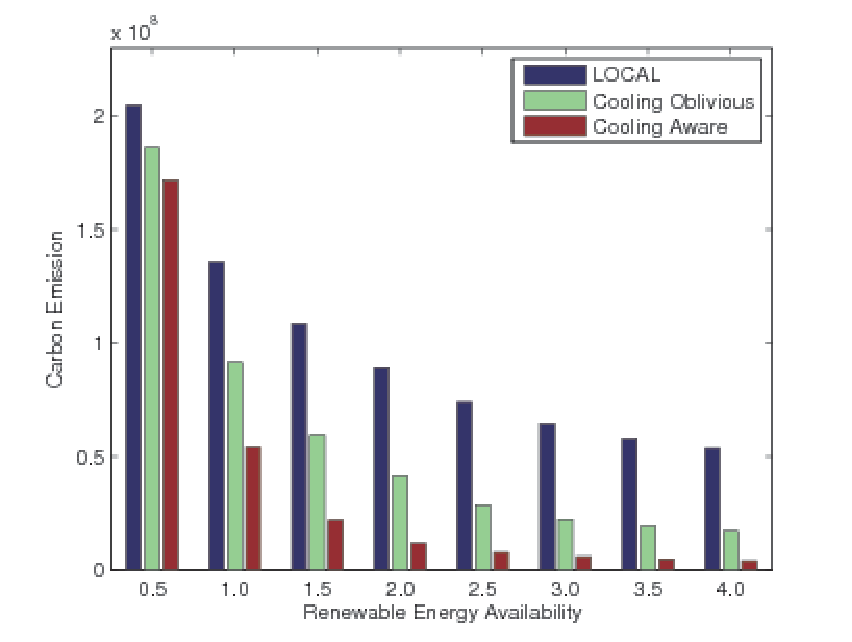
\epsfig{file=carbon_summer.pdf, height=2.2in, width=3.2in}
\caption{Comparison of carbon emission of Cooling-aware GLB, Cooling-oblivious GLB and LOCAL.}
\end{figure}


The geographical load balancing method model exploits variation in energy costs by routing requests to where energy cost is low. When the data centers have on-site renewable energy plants (as in our setting), renewable energy becomes cheap; the model allows optimal usage of these renewables and thus has the desirable side-effect of reducing carbon emissions.

We can estimate the \carbondioxide{} emissions by multiplying the grid energy usage of each data center location by the \carbondioxide{} emission per energy unit. Figure 4 shows the \carbondioxide{} emission comparison of each model in summer. By using the Cooling-aware GLB model, aggregate carbon emissions can be reduced by more than 50\% as compared to LOCAL if the total renewable energy supply is equal to the total IT demand. If more renewable energy is available, the carbon emission of Cooling-aware GLB is even less than half of that of Cooling-oblivious GLB.

The environmental impact of our new model is significant. \carbondioxide{} emissions are reduced even even when firms' optimizations do not consider the environmental externality of \carbondioxide{} emissions. Environmental benefits could be even greater if firms are given incentives to be environmentally friendly.


\subsection{GLB versus Storage}

\begin{figure}
\centering
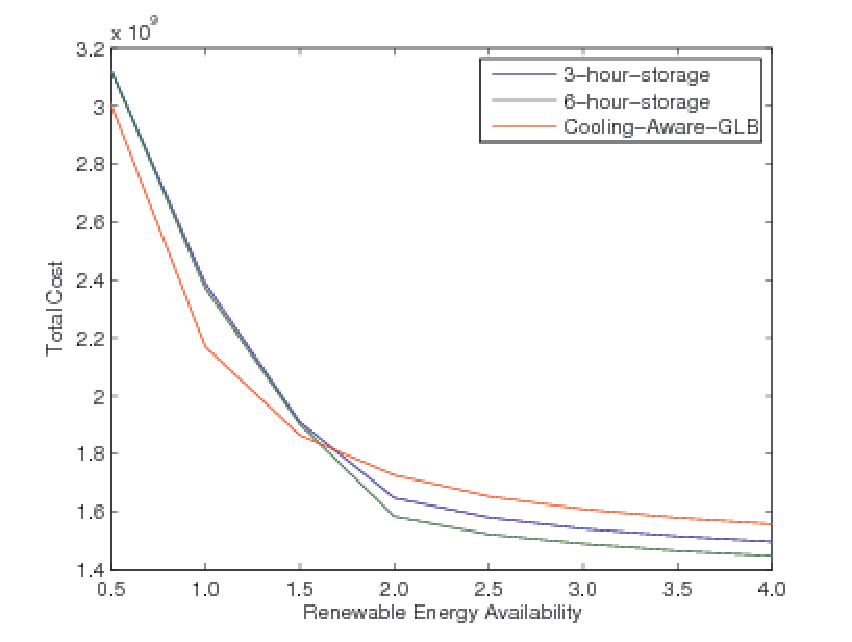
\epsfig{file=cost_storage.pdf, height=2.2in, width=3.2in}
\caption{Comparison of optimal costs of the storage model and the Cooling-aware GLB model.}
\end{figure}
\begin{figure}
\centering
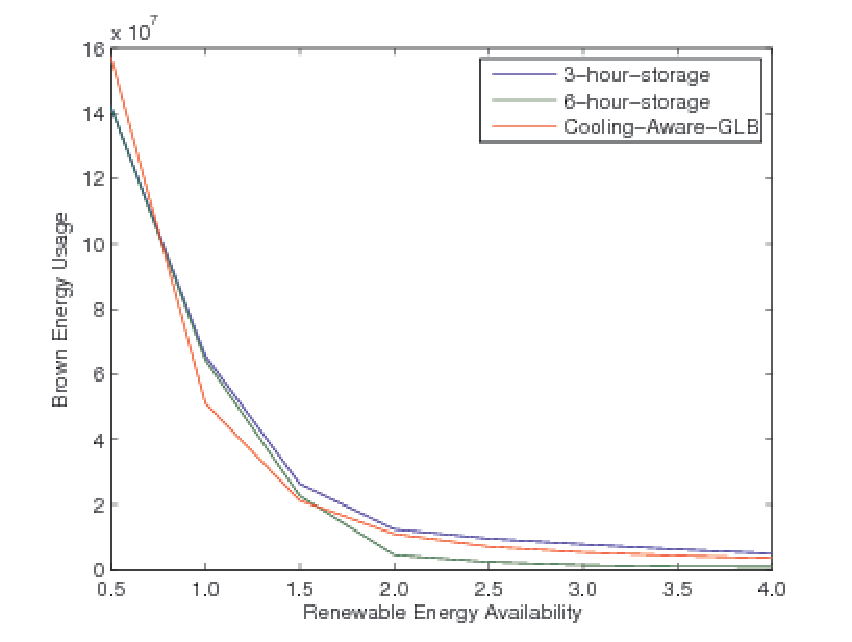
\epsfig{file=brown_storage.pdf, height=2.2in, width=3.2in}
\caption{Comparison of brown energy usage of the storage model and the Cooling-aware GLB model.}
\end{figure}
One alternative way of using renewable energy efficiently is to store the extra renewables at some moments for future use. Whereas applying geographical load balancing adjusts energy demand according to supply in each location, adding energy storage adjusts supply according to demand. We are interested in the performance characteristics of both methods. In this experiment, we compare the cost curve and the brown energy usage curve of using GLB and using storage. Since our experiment starts at midnight, the time when the data centers are likely to have used all of its storage for batch jobs \cite{adam:cooling}, we assume that the storage starts empty.

Figure 5 illustrates the trend of optimal costs of these models with respect to varying renewable availability. It shows that Cooling-aware GLB has lower costs when the total renewable energy is less than 1.5 times the aggregate IT demand, and the storage model is better when renewable energy is in large surplus.

Figure 6 compares brown energy under each model. The result suggests that the Cooling-aware GLB model needs less energy from the grid compared to the 6-hour-storage curve when the total renewable supply is less than 1.5 times of the total IT power demand. Moreover, it needs less grid energy than the total renewable energy compared to the 3-hour-storage model, in almost the entire renewable availability interval, except when the renewable availability coefficient is 0.5. The environmental impact advantage of our new model is even more salient than to the cost advantage.

We thus can conclude that our model is better than the storage model when the renewable generation facilities are not yet built, because it requires less prior infrastructure investment.

\section{Future work}
Our simulation and visualization software can be used to answer questions about extensions to the model that would be useful when putting it into practice, such as—
\begin{itemize}
\item incorporating other kinds of renewables into the model
\item treating data centers as endogenous. In the long run, where should we build new data centers, and what local renewables and energy storage systems do we use?
\item finding the optimal control timescale. It is costly to switch servers on and off, so the current algorithms only change routing every fixed period, which is suboptimal. This significantly restricts the savings that follow-the-renewables routing can yield, but the topic hasn’t yet been explored deeply. Being able to simulate the whole system helps for this.
\item helping discover and then exploit emergent phenomena when looking at systems of many data centers. An example of such a phenomenon deals with the optimal mix of renewable energy for powering data centers. Since the sun shines in the daytime when people are awake and searching the internet, one might expect solar power to dominate. But Wierman’s paper showed that in fact wind is more effective, because its low spatial and temporal correlation is especially useful for geographical load balancing. With solar power, when requests come at night you are forced to buy electricity off the grid, but with wind power, it’s almost always windy somewhere.
\end{itemize}

\bibliographystyle{abbrv}
\bibliography{surfReport}
\end{document}
